\documentclass[11pt]{article}

% =========================
% Packages
% =========================
\usepackage[margin=0.78in]{geometry}
\usepackage{amsmath,amssymb,amsfonts,mathtools}
\usepackage{booktabs,array,tabularx,longtable,multirow}
\usepackage{enumitem}
\usepackage[most]{tcolorbox}
\usepackage{xcolor}
\usepackage{fancyhdr}
\usepackage{titlesec}
\usepackage{hyperref}
\usepackage{lastpage}
\usepackage{setspace}
\usepackage{tikz}
\usepackage{pgfplots}
\usepackage{needspace}
\usepackage{caption}
\usepackage{multicol}
\usepackage{graphicx}
\usepackage{amsthm}
\usepackage{mathrsfs}
\usepackage{bm}
\usepackage{float}
\usepackage{colortbl}
\usepackage{array}
\usepackage{etoolbox}
\usetikzlibrary{calc,arrows.meta,positioning,decorations.pathreplacing,angles,quotes,intersections}

\pgfplotsset{compat=1.18}
\setstretch{1.14}
\setlength{\parindent}{0pt}
\setlength{\parskip}{0.45em}
\setlist[itemize]{leftmargin=1.8em}
\setlist[enumerate]{leftmargin=2em}

% =========================
% Colors
% =========================
\definecolor{novelPurple}{RGB}{98,54,255}
\definecolor{novelPurpleDark}{RGB}{72,34,204}
\definecolor{novelPurpleLight}{RGB}{243,239,255}
\definecolor{novelPurpleLine}{RGB}{165,135,255}
\definecolor{npgray}{RGB}{78,78,78}
\definecolor{softgray}{RGB}{246,246,250}
\definecolor{softlav}{RGB}{249,247,255}
\definecolor{greencheck}{RGB}{24,128,88}
\definecolor{warmred}{RGB}{188,54,54}

% =========================
% Hyperref
% =========================
\hypersetup{
    colorlinks=true,
    linkcolor=novelPurpleDark,
    urlcolor=novelPurpleDark,
    citecolor=novelPurpleDark
}

% =========================
% Header / Footer
% =========================
\pagestyle{fancy}
\fancyhf{}
\fancyhead[L]{\textbf{Novel Prep Learning Center}}
\fancyhead[R]{\textbf{AP Calculus BC --- Unit 9}}
\fancyfoot[C]{\textcolor{novelPurpleDark}{\thepage\ /\ \pageref{LastPage}}}
\renewcommand{\headrulewidth}{0.4pt}
\renewcommand{\footrulewidth}{0pt}

% =========================
% Numbering depth and TOC
% =========================
\setcounter{secnumdepth}{3}
\setcounter{tocdepth}{3}

% =========================
% Section styles
% =========================
\titleformat{\section}
{\Large\bfseries\color{novelPurpleDark}}{\thesection.}{0.6em}{}

\titleformat{\subsection}
{\large\bfseries\color{novelPurple}}{\thesubsection.}{0.6em}{}

\titleformat{\subsubsection}
{\normalsize\bfseries\color{novelPurpleDark}}{\thesubsubsection.}{0.6em}{}

% =========================
% tcolorbox styles
% =========================
\tcbset{
  enhanced,
  sharp corners,
  boxrule=1pt
}

\newtcolorbox{theorybox}[1]{
  colback=white,
  colframe=novelPurple,
  colbacktitle=novelPurple,
  coltitle=white,
  title=\textbf{#1},
  fonttitle=\bfseries,
  sharp corners,
  enhanced,
  breakable
}

\newtcolorbox{notebox}[1]{
  colback=novelPurpleLight,
  colframe=novelPurple,
  colbacktitle=novelPurple,
  coltitle=white,
  title=\textbf{#1},
  fonttitle=\bfseries,
  sharp corners,
  enhanced,
  breakable
}

\newtcolorbox{skillbox}[1]{
  colback=softlav,
  colframe=novelPurpleDark,
  colbacktitle=novelPurpleDark,
  coltitle=white,
  title=\textbf{#1},
  fonttitle=\bfseries,
  sharp corners,
  enhanced,
  breakable
}

\newtcolorbox{summarybox}[1]{
  colback=softgray,
  colframe=novelPurpleDark,
  colbacktitle=novelPurpleDark,
  coltitle=white,
  title=\textbf{#1},
  fonttitle=\bfseries,
  sharp corners,
  enhanced,
  breakable
}

\newtcolorbox{practicebox}[1]{
  colback=white,
  colframe=novelPurpleLine,
  colbacktitle=novelPurpleLine,
  coltitle=black,
  title=\textbf{#1},
  fonttitle=\bfseries,
  sharp corners,
  enhanced,
  breakable
}

\newtcolorbox{homeworkset}[1]{
  colback=white,
  colframe=novelPurpleDark,
  colbacktitle=novelPurpleDark,
  coltitle=white,
  title=\textbf{#1},
  fonttitle=\bfseries,
  sharp corners,
  enhanced,
  breakable,
  boxrule=1pt
}

\newcommand{\hwspace}{\vspace{0.8em}\hrule\vspace{0.8em}}

% =========================
% Commands
% =========================
\newcounter{examplectr}[subsection]
\renewcommand{\theexamplectr}{\thesubsection.\arabic{examplectr}}

\newcommand{\example}[1]{%
\refstepcounter{examplectr}
\Needspace{8\baselineskip}
\noindent{\color{novelPurpleDark}\textbf{Example \theexamplectr.}} \textbf{#1}\par
}

\newcommand{\solution}{\noindent{\textbf{Solution.}}}

\newcommand{\apcheckpoint}[1]{%
\begin{skillbox}{AP Checkpoint}
#1
\end{skillbox}
}

\newcommand{\unitchapter}[1]{%
\newpage
\subsection{#1}
}

\newcommand{\unitsubtopic}[1]{%
\subsubsection{#1}
}

\newcommand{\R}{\mathbb{R}}
\newcommand{\vect}[1]{\mathbf{#1}}

% =========================
% TikZ figures
% =========================
\newcommand{\paramparabolafigure}{
\begin{center}
\begin{tikzpicture}[scale=0.95]
\draw[novelPurpleDark, line width=0.9pt, ->] (-2.5,0) -- (9.5,0) node[right] {$x$};
\draw[novelPurpleDark, line width=0.9pt, ->] (0,-1.8) -- (0,5.5) node[above] {$y$};
\draw[novelPurple, line width=1.25pt, smooth, samples=160, domain=-2:4]
plot ({\x*\x-2*\x},{\x+1});
\foreach \x/\y in {8/-1,3/0,0/1,-1/2,0/3,3/4,8/5}
{
    \fill[novelPurpleDark] (\x,\y) circle (1.8pt);
}
\node[text=npgray] at (5.8,4.8) {\small \(x=t^2-2t,\ y=t+1\)};
\node[text=npgray] at (5.4,4.35) {\small parametric parabola};
\end{tikzpicture}
\end{center}
}

\newcommand{\circleparamfigure}{
\begin{center}
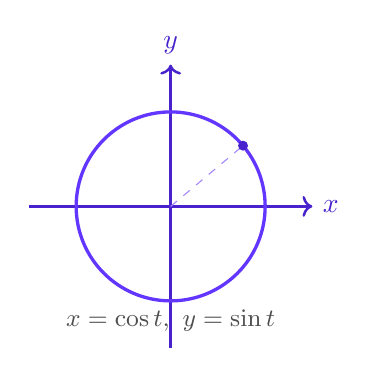
\begin{tikzpicture}[scale=1.0]
\draw[novelPurpleDark, line width=0.9pt, ->] (-1.8,0) -- (1.8,0) node[right] {$x$};
\draw[novelPurpleDark, line width=0.9pt, ->] (0,-1.8) -- (0,1.8) node[above] {$y$};
\draw[novelPurple, line width=1.2pt] (0,0) circle (1.2);
\draw[novelPurpleLine, dashed] (0,0)--(40:1.2);
\fill[novelPurpleDark] (40:1.2) circle (1.8pt);
\node[text=npgray] at (0,-1.45) {\small \(x=\cos t,\ y=\sin t\)};
\end{tikzpicture}
\end{center}
}

\newcommand{\paramtangentfigure}{
\begin{center}
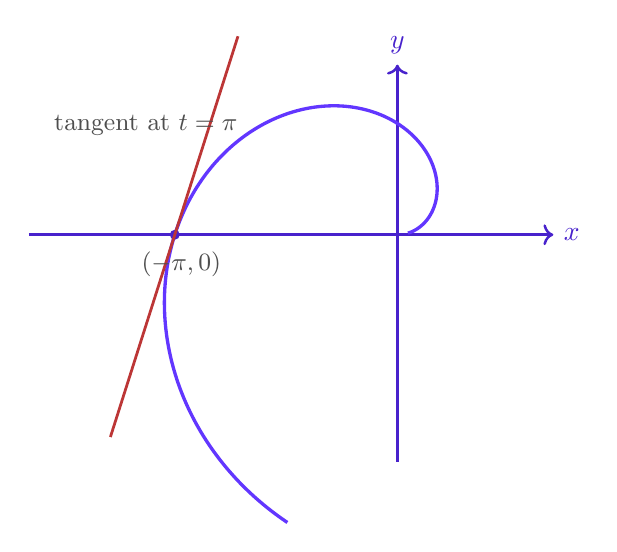
\begin{tikzpicture}[scale=0.9]
    % axes
    \draw[novelPurpleDark, line width=0.9pt, ->] (-5.2,0) -- (2.2,0) node[right] {$x$};
    \draw[novelPurpleDark, line width=0.9pt, ->] (0,-3.2) -- (0,2.4) node[above] {$y$};

    % parametric curve: x=t cos t, y=t sin t
    \draw[novelPurple, line width=1.2pt, smooth, samples=220, domain=0.15:4.35]
        plot ({\x*cos(deg(\x))},{\x*sin(deg(\x))});

    % point at t = pi
    \coordinate (P) at ({pi*cos(180)},{pi*sin(180)});
    \fill[novelPurpleDark] (P) circle (2pt);

    % tangent line at t = pi, slope = pi
    % y = pi(x + pi)
    \draw[warmred, line width=1.0pt]
        (-4.05,{pi*(-4.05 + pi)}) -- (-2.25,{pi*(-2.25 + pi)});

    % labels
    \node[text=npgray] at (-3.55,1.55) {\small tangent at \(t=\pi\)};
    \node[text=npgray] at (-3.05,-0.42) {\small \((-\pi,0)\)};
\end{tikzpicture}
\end{center}
}
\newcommand{\hvparamfigure}{
\begin{center}
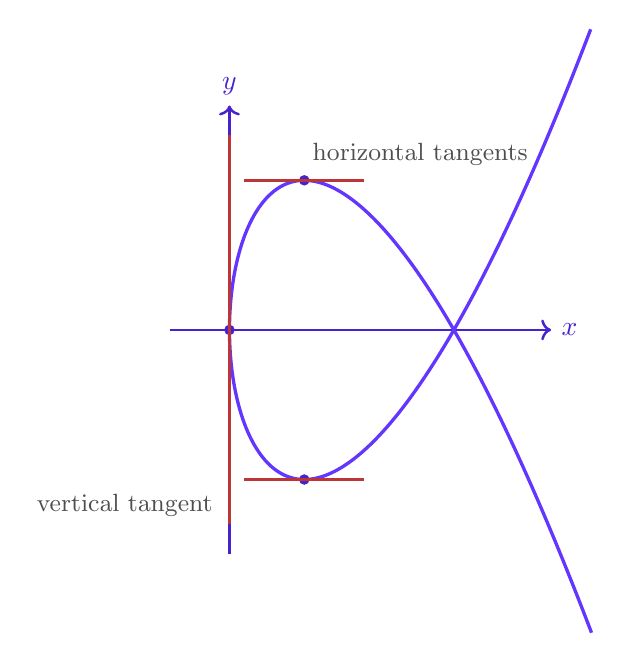
\begin{tikzpicture}[scale=0.95]
\draw[novelPurpleDark, line width=0.9pt, ->] (-0.8,0) -- (4.3,0) node[right] {$x$};
\draw[novelPurpleDark, line width=0.9pt, ->] (0,-3.0) -- (0,3.0) node[above] {$y$};
\draw[novelPurple, line width=1.2pt, smooth, samples=180, domain=-2.2:2.2]
plot ({\x*\x},{\x*\x*\x-3*\x});
\fill[novelPurpleDark] (1,2) circle (2pt);
\fill[novelPurpleDark] (1,-2) circle (2pt);
\fill[novelPurpleDark] (0,0) circle (2pt);
\draw[warmred, line width=1pt] (0.2,2)--(1.8,2);
\draw[warmred, line width=1pt] (0.2,-2)--(1.8,-2);
\draw[warmred, line width=1pt] (0,-2.6)--(0,2.6);
\node[text=npgray] at (2.55,2.35) {\small horizontal tangents};
\node[text=npgray] at (-1.4,-2.35) {\small vertical tangent};
\end{tikzpicture}
\end{center}
}

\newcommand{\secondderivfigure}{
\begin{center}
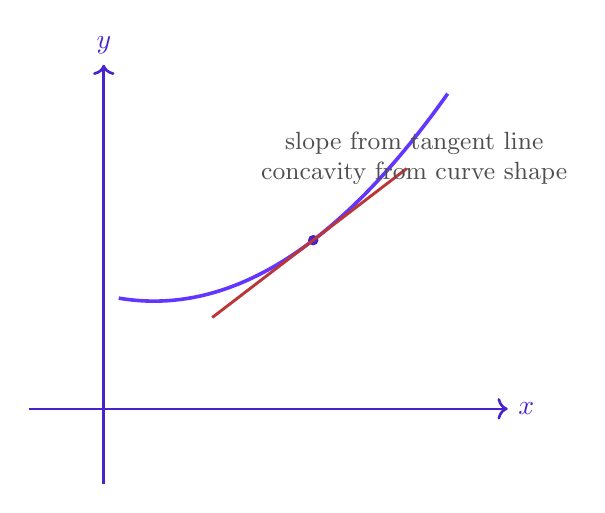
\begin{tikzpicture}[scale=0.95]
    % axes
    \draw[novelPurpleDark, line width=0.95pt, ->] (-1,0) -- (5.4,0) node[right] {$x$};
    \draw[novelPurpleDark, line width=0.95pt, ->] (0,-1) -- (0,4.6) node[above] {$y$};

    % curve: y = 0.18(x-2.2)^2 + 0.55x + 0.65
    \draw[novelPurple, line width=1.3pt, smooth, samples=180, domain=0.2:4.6]
        plot (\x,{0.18*(\x-2.2)^2 + 0.55*\x + 0.65});

    % chosen tangent point x0 = 2.8
    % y0 = 0.18*(2.8-2.2)^2 + 0.55*2.8 + 0.65 = 2.2548
    % slope m = derivative = 0.36(x-2.2)+0.55, so at x=2.8: m = 0.766
    \coordinate (P) at (2.8,2.2548);
    \fill[novelPurpleDark] (P) circle (2pt);

    % tangent line at x = 2.8
    \draw[warmred, line width=1.05pt]
        (1.45,{2.2548 + 0.766*(1.45-2.8)})
        --
        (4.05,{2.2548 + 0.766*(4.05-2.8)});

    % label
    \node[text=npgray, align=left] at (4.15,3.55) {\small slope from tangent line};
    \node[text=npgray, align=left] at (4.15,3.15) {\small concavity from curve shape};
\end{tikzpicture}
\end{center}
}

\newcommand{\vectorfigure}{
\begin{center}
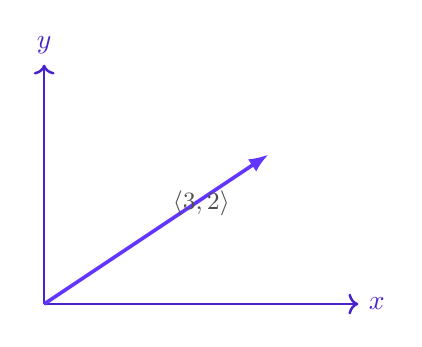
\begin{tikzpicture}[scale=0.95]
\draw[novelPurpleDark, line width=0.9pt, ->] (0,0) -- (4.2,0) node[right] {$x$};
\draw[novelPurpleDark, line width=0.9pt, ->] (0,0) -- (0,3.2) node[above] {$y$};
\draw[-{Latex[length=2.5mm]}, line width=1.3pt, color=novelPurple] (0,0)--(3,2);
\node[text=npgray] at (2.1,1.35) {\small \(\langle 3,2\rangle\)};
\end{tikzpicture}
\end{center}
}

\newcommand{\motionfigure}{
\begin{center}
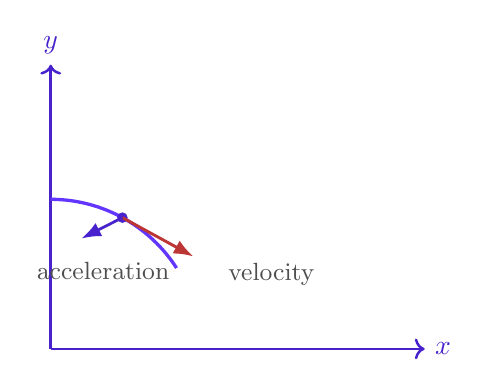
\begin{tikzpicture}[scale=0.95]
\draw[novelPurpleDark, line width=0.9pt, ->] (0,0) -- (5,0) node[right] {$x$};
\draw[novelPurpleDark, line width=0.9pt, ->] (0,0) -- (0,3.8) node[above] {$y$};
\draw[novelPurple, line width=1.2pt, smooth, samples=120, domain=0:2]
plot ({2*sin(deg(\x/2))},{2*cos(deg(\x/2))});
\fill[novelPurpleDark] ({2*sin(deg(1/2))},{2*cos(deg(1/2))}) circle (2pt);
\draw[-{Latex[length=2.5mm]}, warmred, line width=1.05pt] ({2*sin(deg(1/2))},{2*cos(deg(1/2))}) -- +(0.95,-0.52);
\draw[-{Latex[length=2.5mm]}, novelPurpleDark, line width=1.0pt] ({2*sin(deg(1/2))},{2*cos(deg(1/2))}) -- +(-0.55,-0.28);
\node[text=npgray] at (2.95,1.0) {\small velocity};
\node[text=npgray] at (0.7,1.05) {\small acceleration};
\end{tikzpicture}
\end{center}
}

\newcommand{\polargridfigure}{
\begin{center}
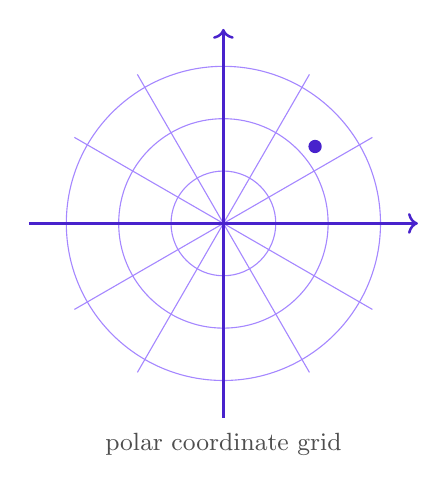
\begin{tikzpicture}[scale=0.95]
\foreach \r in {0.7,1.4,2.1}
  \draw[novelPurpleLine] (0,0) circle (\r);
\foreach \ang in {0,30,...,330}
  \draw[novelPurpleLine] (0,0)--(\ang:2.3);
\draw[novelPurple, line width=1.2pt] (40:1.6) node[circle,fill=novelPurpleDark,inner sep=1.7pt] {};
\draw[novelPurpleDark, line width=0.9pt, ->] (-2.6,0)--(2.6,0);
\draw[novelPurpleDark, line width=0.9pt, ->] (0,-2.6)--(0,2.6);
\node[text=npgray] at (0,-2.95) {\small polar coordinate grid};
\end{tikzpicture}
\end{center}
}

\newcommand{\polarconversionfigure}{
\begin{center}
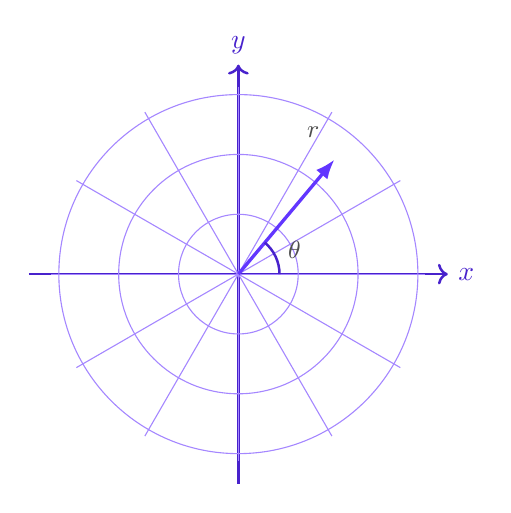
\begin{tikzpicture}[scale=0.95]
\draw[novelPurpleDark, line width=0.9pt, ->] (-2.8,0) -- (2.8,0) node[right] {$x$};
\draw[novelPurpleDark, line width=0.9pt, ->] (0,-2.8) -- (0,2.8) node[above] {$y$};
\foreach \r in {0.8,1.6,2.4}
  \draw[novelPurpleLine] (0,0) circle (\r);
\foreach \ang in {0,30,...,330}
  \draw[novelPurpleLine] (0,0)--(\ang:2.5);
\draw[-{Latex[length=2.5mm]}, novelPurple, line width=1.2pt] (0,0)--(50:2);
\draw[novelPurpleDark, line width=0.9pt] (0.55,0) arc[start angle=0,end angle=50,radius=0.55];
\node[text=npgray] at (1.0,1.9) {\small \(r\)};
\node[text=npgray] at (0.75,0.32) {\small \(\theta\)};
\end{tikzpicture}
\end{center}
}

\newcommand{\polarrosefigure}{
\begin{center}
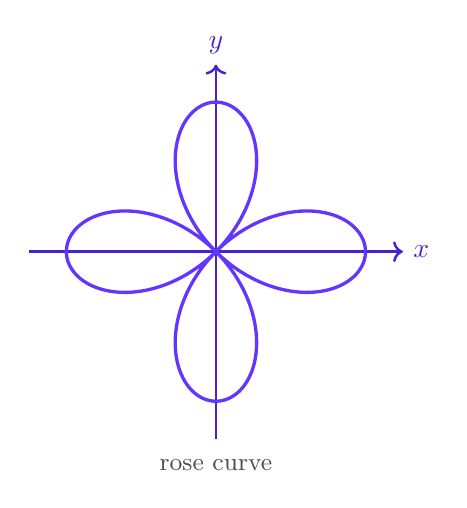
\begin{tikzpicture}[scale=0.95]
\draw[novelPurpleDark, line width=0.9pt, ->] (-2.5,0)--(2.5,0) node[right] {$x$};
\draw[novelPurpleDark, line width=0.9pt, ->] (0,-2.5)--(0,2.5) node[above] {$y$};
\draw[novelPurple, line width=1.2pt, smooth, samples=240, domain=0:6.283]
plot ({cos(deg(\x))*cos(deg(2*\x))*2},{sin(deg(\x))*cos(deg(2*\x))*2});
\node[text=npgray] at (0,-2.85) {\small rose curve};
\end{tikzpicture}
\end{center}
}

\newcommand{\polarareafigure}{
\begin{center}
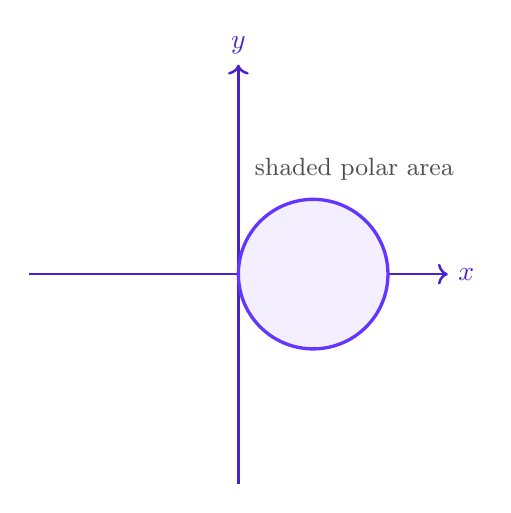
\begin{tikzpicture}[scale=0.95]
\draw[novelPurpleDark, line width=0.9pt, ->] (-2.8,0) -- (2.8,0) node[right] {$x$};
\draw[novelPurpleDark, line width=0.9pt, ->] (0,-2.8) -- (0,2.8) node[above] {$y$};
\fill[novelPurpleLight] (0,0)
  -- plot[smooth, samples=120, domain=-90:90]
  ({2*cos(\x)*cos(\x)},{2*cos(\x)*sin(\x)})
  -- cycle;
\draw[novelPurple, line width=1.2pt, smooth, samples=120, domain=-90:90]
plot ({2*cos(\x)*cos(\x)},{2*cos(\x)*sin(\x)});
\node[text=npgray] at (1.55,1.4) {\small shaded polar area};
\end{tikzpicture}
\end{center}
}

% =========================================================
\begin{document}

\begin{titlepage}
\centering
\vspace*{2.0cm}

{\fontsize{28}{32}\selectfont\bfseries\color{novelPurpleDark} AP Calculus BC\par}
\vspace{0.4cm}
{\fontsize{28}{32}\selectfont\bfseries\color{novelPurpleDark} Unit 9: Parametric, Polar, and Vector-Valued Functions\par}


\vspace{1.0cm}

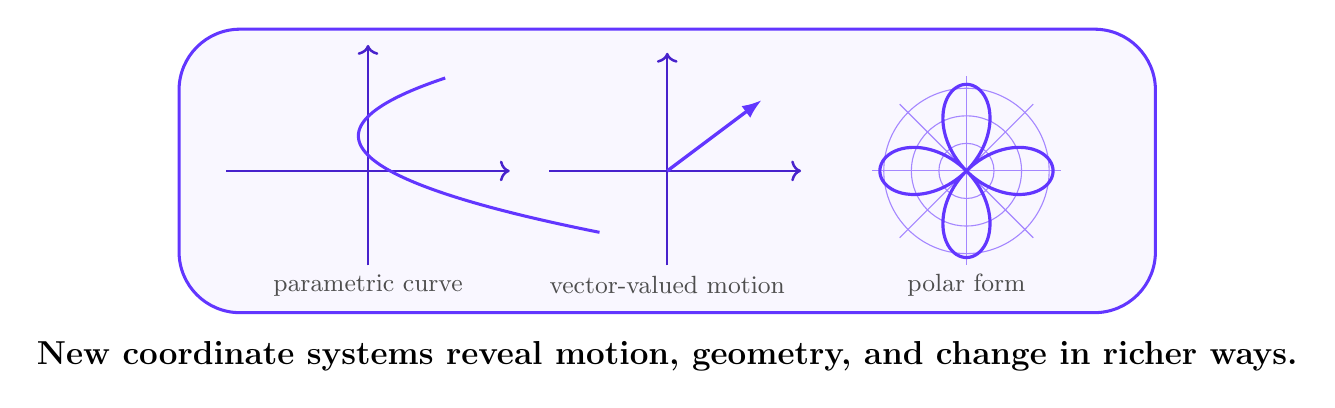
\begin{tikzpicture}[scale=1]
\fill[softlav,rounded corners=22pt] (-6.2,-1.8) rectangle (6.2,1.8);
\draw[novelPurple, line width=1.1pt, rounded corners=22pt] (-6.2,-1.8) rectangle (6.2,1.8);

\begin{scope}[shift={(-3.8,0)}]
\draw[novelPurpleDark, line width=0.9pt, ->] (-1.8,0) -- (1.8,0);
\draw[novelPurpleDark, line width=0.9pt, ->] (0,-1.2) -- (0,1.6);
\draw[novelPurple, line width=1.1pt, smooth, samples=120, domain=-1.4:1.4]
plot ({\x*\x-0.7*\x},{0.7*\x+0.2});
\node[text=npgray] at (0,-1.45) {\small parametric curve};
\end{scope}

\begin{scope}[shift={(0,0)}]
\draw[novelPurpleDark, line width=0.9pt, ->] (-1.5,0) -- (1.7,0);
\draw[novelPurpleDark, line width=0.9pt, ->] (0,-1.2) -- (0,1.5);
\draw[-{Latex[length=2.5mm]}, line width=1.2pt, color=novelPurple] (0,0)--(1.2,0.9);
\node[text=npgray] at (0,-1.45) {\small vector-valued motion};
\end{scope}

\begin{scope}[shift={(3.8,0)}]
\foreach \r in {0.35,0.7,1.05}
  \draw[novelPurpleLine] (0,0) circle (\r);
\foreach \ang in {0,45,...,315}
  \draw[novelPurpleLine] (0,0)--(\ang:1.2);
\draw[novelPurple, line width=1.15pt, smooth, samples=200, domain=0:6.283]
plot ({cos(deg(\x))*cos(deg(2*\x))*1.1},{sin(deg(\x))*cos(deg(2*\x))*1.1});
\node[text=npgray] at (0,-1.45) {\small polar form};
\end{scope}

\node[align=center] at (0,-2.35) {\large\bfseries New coordinate systems reveal motion, geometry, and change in richer ways.};
\end{tikzpicture}

\vfill

\begin{minipage}{0.84\textwidth}
\begin{notebox}{Design Goals for This Revision}
\begin{itemize}
    \item Keep the full Unit 9 scope from your original chapter.
    \item Use the same polished Novel Prep visual system as the finalized Unit 10 version.
    \item Clarify the links among parametric, vector-valued, and polar descriptions.
    \item Add cleaner diagrams, clearer examples, guided practice, homework, and answer key.
\end{itemize}
\end{notebox}
\end{minipage}

\vfill

{\large\textbf{Novel Prep Learning Center}}\\[0.25em]
{\large Hongjun Zeng}

\end{titlepage}

\tableofcontents
\newpage

\setcounter{section}{8}
\section{Parametric Equations, Polar Coordinates, and Vector-Valued Functions}

\begin{theorybox}{Big Idea}
A graph does not always have to be written as \(y=f(x)\).  
Sometimes the most natural way to describe a curve or a motion is by:
\begin{itemize}
    \item using a parameter \(t\),
    \item using vectors,
    \item or using polar coordinates \((r,\theta)\).
\end{itemize}
This unit extends calculus into these richer coordinate languages.
\end{theorybox}

\begin{notebox}{Teaching Philosophy for This Unit}
Students should see Unit 9 as a change of language, not a change of calculus.
The same big ideas keep appearing:
\[
\text{position} \to \text{slope} \to \text{derivative} \to \text{accumulation} \to \text{geometry}.
\]
The formulas look different, but the calculus meaning is the same.
\end{notebox}

\begin{theorybox}{Core Idea}
Parametric equations, vector-valued functions, and polar equations all describe curves in alternative ways.
The central questions stay the same:
\begin{itemize}
    \item Where is the object?
    \item How fast is it changing?
    \item What is the slope?
    \item What is the length?
    \item What area is enclosed?
\end{itemize}
\end{theorybox}

\apcheckpoint{
In Unit 9, always ask:
\begin{itemize}
    \item What is the independent parameter?
    \item Which derivative formula matches this representation?
    \item Am I finding displacement, total distance, speed, geometric length, or area?
\end{itemize}
}

\begin{theorybox}{AP Unit 9 Topic Map}
\renewcommand{\arraystretch}{1.25}
\begin{tabularx}{\textwidth}{@{}p{0.20\textwidth}p{0.30\textwidth}X@{}}
\toprule
Topic & Focus & Main Skill Emphasis \\
\midrule
9.1 Parametric Equations & define curves with a parameter & eliminate parameters and find slopes \\
9.2 Second Derivatives (Parametric) & curvature and concavity & compute \(\dfrac{d^2y}{dx^2}\) correctly \\
9.3 Arc Length of Parametric Curves & geometric length and speed & apply length formulas carefully \\
9.4 Vector-Valued Functions & vector notation for motion & differentiate componentwise \\
9.5 Integrating Vector-Valued Functions & accumulation in vector form & integrate componentwise \\
9.6 Motion Problems & displacement, distance, velocity, acceleration & connect derivatives to physical meaning \\
9.7 Polar Coordinates & new coordinate system & convert and differentiate in polar form \\
9.8 Area of One Polar Curve & enclosed area & use the polar area formula \\
9.9 Area Between Two Polar Curves & comparison of radii & set up correct area bounds \\
\bottomrule
\end{tabularx}
\end{theorybox}

% =========================================================
\unitchapter{Defining and Differentiating Parametric Equations}

\unitsubtopic{Parametric Equations}

\begin{theorybox}{Definition of Parametric Equations}
A curve can be described by writing both \(x\) and \(y\) as functions of a third variable \(t\):
\[
x=f(t),\qquad y=g(t).
\]
The variable \(t\) is called the \textbf{parameter}. Each value of \(t\) determines a point \((x,y)\) on the curve.
\end{theorybox}

\paramparabolafigure

\example{Sketch and identify the parametric curve}
Sketch and identify the curve defined by
\[
x=t^2-2t,\qquad y=t+1.
\]

\solution
From
\[
y=t+1,
\]
we get
\[
t=y-1.
\]
Substitute into \(x\):
\[
x=(y-1)^2-2(y-1)=y^2-4y+3.
\]
So the curve is a parabola opening to the right.

\example{Unit circle in parametric form}
Identify the curve
\[
x=\cos t,\qquad y=\sin t,\qquad 0\le t\le 2\pi.
\]

\solution
Square and add:
\[
x^2+y^2=\cos^2 t+\sin^2 t=1.
\]
Therefore the curve is the unit circle centered at the origin.

\circleparamfigure

\unitsubtopic{Differentiating Parametric Equations}

\begin{theorybox}{Derivative of a Parametric Curve}
If
\[
x=f(t),\qquad y=g(t),
\]
then the slope of the tangent line is
\[
\frac{dy}{dx}=\frac{\frac{dy}{dt}}{\frac{dx}{dt}},
\qquad \text{provided } \frac{dx}{dt}\ne 0.
\]
\end{theorybox}

\paramtangentfigure

\example{Eliminate the parameter}
Given
\[
x=e^{-t},\qquad y=e^{2t}-1,
\]
eliminate the parameter and write the rectangular equation.

\solution
Take the natural log of \(x=e^{-t}\):
\[
\ln x=-t \quad\Longrightarrow\quad t=-\ln x.
\]
Substitute into \(y\):
\[
y=e^{2(-\ln x)}-1=e^{-\ln(x^2)}-1=\frac{1}{x^2}-1,
\qquad x>0.
\]

\example{Tangent line to a parametric curve}
Given
\[
x=t\cos t,\qquad y=t\sin t,
\]
find the tangent line at \(t=\pi\).

\solution
Differentiate:
\[
\frac{dx}{dt}=\cos t-t\sin t,\qquad
\frac{dy}{dt}=\sin t+t\cos t.
\]
Thus
\[
\frac{dy}{dx}
=
\frac{\sin t+t\cos t}{\cos t-t\sin t}.
\]
At \(t=\pi\),
\[
x=-\pi,\qquad y=0,
\]
and
\[
\frac{dy}{dx}
=
\frac{0+\pi(-1)}{-1-0}
=
\pi.
\]
Therefore the tangent line is
\[
y=\pi(x+\pi).
\]

\hvparamfigure

\example{Horizontal and vertical tangents}
Let
\[
x=t^2,\qquad y=t^3-3t.
\]
Find the points where the tangent line is horizontal or vertical.

\solution
Differentiate:
\[
\frac{dx}{dt}=2t,\qquad \frac{dy}{dt}=3t^2-3.
\]
A horizontal tangent occurs when
\[
\frac{dy}{dt}=0 \quad\text{and}\quad \frac{dx}{dt}\ne 0.
\]
So
\[
3t^2-3=0 \Longrightarrow t=\pm 1.
\]
At \(t=1\), the point is \((1,-2)\).  
At \(t=-1\), the point is \((1,2)\).

A vertical tangent occurs when
\[
\frac{dx}{dt}=0 \quad\text{and}\quad \frac{dy}{dt}\ne 0.
\]
So \(t=0\), giving the point \((0,0)\).

% =========================================================
\unitchapter{Second Derivatives of Parametric Equations}

\begin{theorybox}{Second Derivative of a Parametric Curve}
If
\[
\frac{dy}{dx}=\frac{\frac{dy}{dt}}{\frac{dx}{dt}},
\]
then
\[
\frac{d^2y}{dx^2}
=
\frac{\frac{d}{dt}\left(\frac{dy}{dx}\right)}{\frac{dx}{dt}}.
\]
\end{theorybox}

\secondderivfigure

\example{Find the second derivative of a parametric equation}
Given
\[
x=3t^2-1,\qquad y=\ln t,
\]
find
\[
\frac{d^2y}{dx^2}.
\]

\solution
First,
\[
\frac{dx}{dt}=6t,\qquad \frac{dy}{dt}=\frac1t.
\]
So
\[
\frac{dy}{dx}
=
\frac{1/t}{6t}
=
\frac{1}{6t^2}.
\]
Differentiate with respect to \(t\):
\[
\frac{d}{dt}\left(\frac{1}{6t^2}\right)
=
-\frac{1}{3t^3}.
\]
Now divide by \(\frac{dx}{dt}=6t\):
\[
\frac{d^2y}{dx^2}
=
\frac{-\frac{1}{3t^3}}{6t}
=
-\frac{1}{18t^4}.
\]

\example{Slope and concavity at a specific parameter value}
Given
\[
x=\theta-\cos\theta,\qquad y=1-\sin\theta,
\]
find the slope and concavity at \(\theta=\pi\).

\solution
First,
\[
\frac{dx}{d\theta}=1+\sin\theta,\qquad
\frac{dy}{d\theta}=-\cos\theta.
\]
Thus
\[
\frac{dy}{dx}
=
\frac{-\cos\theta}{1+\sin\theta}.
\]
At \(\theta=\pi\),
\[
\frac{dy}{dx}=1.
\]
Differentiating again and dividing by \(\frac{dx}{d\theta}\), we get
\[
\frac{d^2y}{dx^2}=1,
\]
so the curve is concave up there.

\example{Practice with a parametric curve}
A curve \(C\) is defined by
\[
x=t^2,\qquad y=t^3-3t.
\]
\begin{enumerate}
    \item Show that \(C\) has two tangents at \((3,0)\), and find their equations.
    \item Find the points where the tangent is horizontal or vertical.
\end{enumerate}

\solution
Since \(x=3\) when \(t=\pm\sqrt3\), and in both cases
\[
y=t(t^2-3)=0,
\]
the point \((3,0)\) occurs for two parameter values.

The slope is
\[
\frac{dy}{dx}=\frac{3t^2-3}{2t}.
\]
At \(t=\sqrt3\),
\[
\frac{dy}{dx}=\sqrt3,
\]
and at \(t=-\sqrt3\),
\[
\frac{dy}{dx}=-\sqrt3.
\]
So the two tangent lines are
\[
y=\sqrt3(x-3)
\qquad\text{and}\qquad
y=-\sqrt3(x-3).
\]

Horizontal tangents occur at \(t=\pm1\), giving \((1,-2)\) and \((1,2)\).  
A vertical tangent occurs at \(t=0\).

% =========================================================
\unitchapter{Finding Arc Lengths of Curves Given by Parametric Equations}

\unitsubtopic{Arc Length of a Curve}

\begin{theorybox}{Arc Length Formula for \(y=f(x)\)}
If \(f'(x)\) is continuous on \([a,b]\), then the arc length of \(y=f(x)\) from \(x=a\) to \(x=b\) is
\[
L=\int_a^b \sqrt{1+\left(\frac{dy}{dx}\right)^2}\,dx.
\]
\end{theorybox}

\example{Arc length in rectangular form}
Find the arc length of
\[
y=x^{3/2}
\]
from \(x=1\) to \(x=4\).

\solution
Differentiate:
\[
\frac{dy}{dx}=\frac32 x^{1/2}.
\]
Then
\[
L=\int_1^4 \sqrt{1+\left(\frac32 x^{1/2}\right)^2}\,dx
=
\int_1^4 \sqrt{1+\frac94 x}\,dx.
\]

\unitsubtopic{Arc Length of Parametric Curves}

\begin{theorybox}{Arc Length of a Parametric Curve}
If
\[
x=f(t),\qquad y=g(t),\qquad \alpha\le t\le \beta,
\]
then the arc length is
\[
L=\int_\alpha^\beta \sqrt{\left(\frac{dx}{dt}\right)^2+\left(\frac{dy}{dt}\right)^2}\,dt.
\]
\end{theorybox}

\example{Arc length of a parametric curve}
For
\[
x=\cos t,\qquad y=\sin t,\qquad 0\le t\le 2\pi,
\]
find the arc length.

\solution
Differentiate:
\[
\frac{dx}{dt}=-\sin t,\qquad \frac{dy}{dt}=\cos t.
\]
So
\[
L=\int_0^{2\pi}\sqrt{\sin^2 t+\cos^2 t}\,dt
=\int_0^{2\pi}1\,dt
=2\pi.
\]

\example{Speed from parametric equations}
The position of a particle is given by
\[
x=2t+3,\qquad y=4t^2,\qquad t\ge 0.
\]
Find the speed when the particle is at the point \((5,4)\).

\solution
The point \((5,4)\) occurs when
\[
2t+3=5 \Longrightarrow t=1,
\]
and indeed \(y=4(1)^2=4\).

Now compute speed:
\[
v(t)=\sqrt{\left(\frac{dx}{dt}\right)^2+\left(\frac{dy}{dt}\right)^2}
=
\sqrt{2^2+(8t)^2}.
\]
At \(t=1\),
\[
v(1)=\sqrt{4+64}=\sqrt{68}=2\sqrt{17}.
\]

% =========================================================
\unitchapter{Defining and Differentiating Vector-Valued Functions}

\unitsubtopic{Vector}

\begin{theorybox}{Definition of a Vector}
A vector is a quantity with both magnitude and direction.  
In two dimensions, a vector may be written as
\[
\langle v_1,v_2\rangle.
\]
Its magnitude is
\[
\|\vect{v}\|=\sqrt{v_1^2+v_2^2}.
\]
\end{theorybox}

\vectorfigure

\example{Magnitude and direction of a vector}
Consider the vector
\[
\vect{v}=\langle 6,8\rangle.
\]
Find its magnitude.

\solution
\[
\|\vect{v}\|=\sqrt{6^2+8^2}=\sqrt{36+64}=10.
\]
The vector points from the origin to \((6,8)\).

\unitsubtopic{Vector-Valued Functions}

\begin{theorybox}{Vector-Valued Function}
A function of the form
\[
\vect{r}(t)=\langle f(t),g(t)\rangle
\]
or
\[
\vect{r}(t)=\langle f(t),g(t),h(t)\rangle
\]
is called a vector-valued function.
It records position as a function of the parameter \(t\).
\end{theorybox}

\begin{theorybox}{Differentiation of Vector-Valued Functions}
Differentiate componentwise:
\[
\vect{r}'(t)=\langle f'(t),g'(t)\rangle
\]
or
\[
\vect{r}'(t)=\langle f'(t),g'(t),h'(t)\rangle.
\]
\end{theorybox}

\example{Derivative of a vector-valued function}
Given
\[
\vect{r}(t)=\langle 4t^2,7t^7\rangle,
\]
find \(\vect{r}'(4)\).

\solution
Differentiate componentwise:
\[
\vect{r}'(t)=\langle 8t,49t^6\rangle.
\]
Then
\[
\vect{r}'(4)=\langle 32,49\cdot 4^6\rangle=\langle 32,200704\rangle.
\]

\example{Vector function and the corresponding plane curve}
For
\[
\vect{r}(t)=\langle t,t^2+2\rangle,
\]
find \(\vect{r}'(t)\), and identify the corresponding rectangular curve.

\solution
\[
\vect{r}'(t)=\langle 1,2t\rangle.
\]
Since \(x=t\) and \(y=t^2+2\), the rectangular equation is
\[
y=x^2+2.
\]
At \(t=1\),
\[
\vect{r}(1)=\langle 1,3\rangle,\qquad \vect{r}'(1)=\langle 1,2\rangle.
\]
\newpage
\begin{theorybox}{Properties of the Derivative}
Let \(\vect{r}(t)\) and \(\vect{u}(t)\) be differentiable vector-valued functions, let \(w(t)\) be a differentiable real-valued function, and let \(c\) be a constant. Then:
\begin{enumerate}
    \item \(\dfrac{d}{dt}[c\vect{r}(t)] = c\vect{r}'(t)\)
    \item \(\dfrac{d}{dt}[\vect{r}(t)\pm \vect{u}(t)] = \vect{r}'(t)\pm \vect{u}'(t)\)
    \item \(\dfrac{d}{dt}[w(t)\vect{r}(t)] = w(t)\vect{r}'(t)+w'(t)\vect{r}(t)\)
    \item \(\dfrac{d}{dt}[\vect{r}(t)\cdot \vect{u}(t)] = \vect{r}(t)\cdot \vect{u}'(t)+\vect{r}'(t)\cdot \vect{u}(t)\)
    \item \(\dfrac{d}{dt}[\vect{r}(w(t))] = \vect{r}'(w(t))\,w'(t)\)
\end{enumerate}
If
\[
\vect{r}(t)\cdot \vect{r}(t)=c
\]
for a constant \(c\), then
\[
\vect{r}(t)\cdot \vect{r}'(t)=0.
\]
\end{theorybox}

\example{Using the derivative of a dot product}
If
\[
\vect{r}(t)=\left\langle \frac1t,-1,\ln t\right\rangle,
\qquad
\vect{u}(t)=\langle t^2,-2t,1\rangle,
\]
find
\[
\frac{d}{dt}\big(\vect{r}(t)\cdot \vect{u}(t)\big).
\]

\solution
First compute the derivatives:
\[
\vect{r}'(t)=\left\langle -\frac1{t^2},0,\frac1t\right\rangle,
\qquad
\vect{u}'(t)=\langle 2t,-2,0\rangle.
\]
Now use the product rule for the dot product:
\[
\frac{d}{dt}\big(\vect{r}\cdot \vect{u}\big)=\vect{r}'\cdot \vect{u}+\vect{r}\cdot \vect{u}'.
\]
Compute each term:
\[
\vect{r}'\cdot \vect{u}
=
\left(-\frac1{t^2}\right)(t^2)+0(-2t)+\left(\frac1t\right)(1)
=
-1+\frac1t,
\]
\[
\vect{r}\cdot \vect{u}'
=
\left(\frac1t\right)(2t)+(-1)(-2)+(\ln t)(0)
=
2+2=4.
\]
So
\[
\frac{d}{dt}\big(\vect{r}(t)\cdot \vect{u}(t)\big)=3+\frac1t.
\]

% =========================================================
\unitchapter{Integrating Vector-Valued Functions}

\begin{theorybox}{Integrating Vector-Valued Functions}
Integrate componentwise:
\[
\int \langle f(t),g(t)\rangle\,dt
=
\left\langle \int f(t)\,dt,\int g(t)\,dt \right\rangle+\vect{C}.
\]
Similarly in three dimensions.
\end{theorybox}

\example{Basic antiderivative}
Find
\[
\int \langle 2t,3t^2\rangle\,dt.
\]

\solution
Integrate each component:
\[
\int \langle 2t,3t^2\rangle\,dt
=
\langle t^2,t^3\rangle+\vect{C}.
\]

\example{Position from velocity}
A particle has velocity
\[
\vect{v}(t)=\langle 2,6t\rangle
\]
and initial position
\[
\vect{r}(0)=\langle 3,1\rangle.
\]
Find \(\vect{r}(t)\).

\solution
Integrate:
\[
\vect{r}(t)=\langle 2t,3t^2\rangle+\vect{C}.
\]
Use the initial condition:
\[
\vect{r}(0)=\langle 0,0\rangle+\vect{C}=\langle 3,1\rangle.
\]
So
\[
\vect{C}=\langle 3,1\rangle,
\]
and therefore
\[
\vect{r}(t)=\langle 2t+3,3t^2+1\rangle.
\]

% =========================================================
\unitchapter{Solving Motion Problems Using Parametric and Vector-Valued Functions}

\unitsubtopic{Motion Terms}

\begin{theorybox}{Key Motion Vocabulary}
If \(\vect{r}(t)\) is position, then:
\[
\vect{v}(t)=\vect{r}'(t)
\quad\text{is velocity,}
\]
\[
\vect{a}(t)=\vect{v}'(t)=\vect{r}''(t)
\quad\text{is acceleration.}
\]
The speed is
\[
\|\vect{v}(t)\|.
\]
The displacement from \(t=a\) to \(t=b\) is
\[
\vect{r}(b)-\vect{r}(a).
\]
The total distance traveled from \(t=a\) to \(t=b\) is
\[
\int_a^b \|\vect{v}(t)\|\,dt.
\]
\end{theorybox}

\unitsubtopic{Calculus with Vector-Valued Functions}

\motionfigure

\example{Velocity, speed, and acceleration on circular motion}
Consider
\[
\vect{r}(t)=\left\langle 2\sin\frac{t}{2},\,2\cos\frac{t}{2}\right\rangle.
\]
Find the velocity, speed, acceleration, and the rectangular equation of the motion.

\solution
Differentiate:
\[
\vect{v}(t)=\left\langle \cos\frac{t}{2},-\sin\frac{t}{2}\right\rangle.
\]
Then the speed is
\[
\|\vect{v}(t)\|
=
\sqrt{\cos^2\frac{t}{2}+\sin^2\frac{t}{2}}
=
1.
\]
Differentiate again:
\[
\vect{a}(t)=\left\langle -\frac12\sin\frac{t}{2},-\frac12\cos\frac{t}{2}\right\rangle.
\]
Also,
\[
x=2\sin\frac{t}{2},\qquad y=2\cos\frac{t}{2}.
\]
So
\[
x^2+y^2=4.
\]

\example{Displacement and total distance}
A particle moves with position
\[
\vect{r}(t)=\langle t^2,\,2t\rangle,\qquad 0\le t\le 2.
\]
Find the displacement and the total distance traveled.

\solution
Displacement:
\[
\vect{r}(2)-\vect{r}(0)=\langle 4,4\rangle-\langle 0,0\rangle=\langle 4,4\rangle.
\]

Velocity:
\[
\vect{v}(t)=\langle 2t,2\rangle.
\]
So the speed is
\[
\|\vect{v}(t)\|=\sqrt{(2t)^2+2^2}=2\sqrt{t^2+1}.
\]
Thus the total distance traveled is
\[
\int_0^2 2\sqrt{t^2+1}\,dt.
\]

\unitsubtopic{Calculus with Parametric Functions}

\example{Slope at a time}
A particle moves according to
\[
x(t)=t^2,\qquad y(t)=t^3-3t.
\]
Find the slope of the path at \(t=2\).

\solution
\[
\frac{dx}{dt}=2t,\qquad \frac{dy}{dt}=3t^2-3.
\]
So
\[
\frac{dy}{dx}=\frac{3t^2-3}{2t}.
\]
At \(t=2\),
\[
\frac{dy}{dx}=\frac{12-3}{4}=\frac94.
\]

\example{Speed from parametric motion}
A particle has position
\[
x=2t+3,\qquad y=4t^2.
\]
Find the speed when the particle is at \((5,4)\).

\solution
At the point \((5,4)\), we have
\[
2t+3=5 \Longrightarrow t=1.
\]
Then
\[
v(t)=\sqrt{\left(\frac{dx}{dt}\right)^2+\left(\frac{dy}{dt}\right)^2}
=
\sqrt{2^2+(8t)^2}.
\]
At \(t=1\),
\[
v(1)=2\sqrt{17}.
\]

\example{Displacement versus total distance in parametric motion}
A particle moves according to
\[
x=t,\qquad y=t^2-2t,\qquad 0\le t\le 3.
\]
Write formulas for the displacement and total distance traveled.

\solution
The position vector is
\[
\vect{r}(t)=\langle t,t^2-2t\rangle.
\]
So the displacement on \([0,3]\) is
\[
\vect{r}(3)-\vect{r}(0)=\langle 3,3\rangle-\langle 0,0\rangle=\langle 3,3\rangle.
\]
Velocity:
\[
\vect{v}(t)=\left\langle 1,2t-2\right\rangle.
\]
Hence the total distance traveled is
\[
\int_0^3 \sqrt{1+(2t-2)^2}\,dt.
\]

% =========================================================
\unitchapter{Polar Coordinates and Differentiating in Polar Form}

\unitsubtopic{Polar Coordinates}

\begin{theorybox}{Polar Coordinates}
In polar coordinates, a point is written as
\[
(r,\theta),
\]
where \(r\) is the directed distance from the origin and \(\theta\) is the angle from the positive \(x\)-axis.
\end{theorybox}

\polargridfigure
\polarconversionfigure

\example{Reading polar coordinates}
Describe what the point \((2,\pi)\) means in polar form.

\solution
It means move a distance \(2\) from the origin in the direction \(\theta=\pi\), which is the negative \(x\)-axis. So the rectangular coordinates are \((-2,0)\).

\unitsubtopic{Coordinate Conversion}

\begin{theorybox}{Coordinate Conversion}
Polar to rectangular:
\[
x=r\cos\theta,\qquad y=r\sin\theta.
\]
Rectangular to polar:
\[
r^2=x^2+y^2,\qquad \tan\theta=\frac{y}{x}.
\]
\end{theorybox}

\example{Polar to rectangular}
Convert
\[
(r,\theta)=(\sqrt3,\pi/6)
\]
to rectangular coordinates.

\solution
\[
x=r\cos\theta=\sqrt3\cdot\frac{\sqrt3}{2}=\frac32,
\qquad
y=r\sin\theta=\sqrt3\cdot\frac12=\frac{\sqrt3}{2}.
\]

\example{Rectangular to polar}
Convert \((-1,1)\) to polar coordinates.

\solution
\[
r=\sqrt{(-1)^2+1^2}=\sqrt2.
\]
Since the point is in Quadrant II,
\[
\theta=\frac{3\pi}{4}.
\]
So the polar coordinates are
\[
\left(\sqrt2,\frac{3\pi}{4}\right).
\]

\example{Converting a polar equation to Cartesian form}
Convert
\[
r=4\sin\theta
\]
to Cartesian form.

\solution
Multiply both sides by \(r\):
\[
r^2=4r\sin\theta.
\]
Then use
\[
r^2=x^2+y^2,\qquad r\sin\theta=y.
\]
So
\[
x^2+y^2=4y.
\]

\unitsubtopic{Derivatives of Polar Functions}

\begin{theorybox}{Derivatives of Polar Functions}
When working with polar functions of the form \(r=f(\theta)\):
\begin{itemize}
    \item \(\dfrac{dr}{d\theta}\) is the rate of change of the radial distance with respect to \(\theta\).
    \item To find \(\dfrac{dr}{d\theta}\), differentiate \(r=f(\theta)\) as you would any ordinary function.
\end{itemize}
To compute the slope of the polar curve, write
\[
x=r\cos\theta,\qquad y=r\sin\theta.
\]
Then
\[
\frac{dx}{d\theta}=\frac{dr}{d\theta}\cos\theta-r\sin\theta,
\qquad
\frac{dy}{d\theta}=\frac{dr}{d\theta}\sin\theta+r\cos\theta.
\]
Hence
\[
\frac{dy}{dx}
=
\frac{\frac{dy}{d\theta}}{\frac{dx}{d\theta}}.
\]
\end{theorybox}

\example{Differentiate a polar function}
If
\[
r=\sin\theta,
\]
find
\[
\frac{dr}{d\theta}.
\]

\solution
Differentiate directly:
\[
\frac{dr}{d\theta}=\cos\theta.
\]

\unitsubtopic{Slope and Tangent Lines}

\example{Slope of a polar curve}
For
\[
r=1+\cos\theta,
\]
find \(\frac{dy}{dx}\) at \(\theta=\frac{\pi}{2}\).

\solution
First,
\[
\frac{dr}{d\theta}=-\sin\theta.
\]
At \(\theta=\frac{\pi}{2}\),
\[
r=1,\qquad \frac{dr}{d\theta}=-1.
\]
Now
\[
\frac{dx}{d\theta}=\frac{dr}{d\theta}\cos\theta-r\sin\theta
=
(-1)(0)-1(1)=-1,
\]
\[
\frac{dy}{d\theta}=\frac{dr}{d\theta}\sin\theta+r\cos\theta
=
(-1)(1)+1(0)=-1.
\]
Therefore
\[
\frac{dy}{dx}=1.
\]

\polarrosefigure

\example{Horizontal and vertical tangents in polar form}
For
\[
r=\sin\theta,
\]
find the points where the tangent line is horizontal or vertical.

\solution
Write
\[
x=r\cos\theta=\sin\theta\cos\theta,\qquad
y=r\sin\theta=\sin^2\theta.
\]
Differentiate:
\[
\frac{dx}{d\theta}=\cos2\theta,\qquad
\frac{dy}{d\theta}=\sin2\theta.
\]

A horizontal tangent occurs when
\[
\frac{dy}{d\theta}=0
\quad\text{and}\quad
\frac{dx}{d\theta}\ne 0.
\]
So
\[
\sin2\theta=0 \Longrightarrow \theta=0,\frac{\pi}{2},\pi.
\]

A vertical tangent occurs when
\[
\frac{dx}{d\theta}=0
\quad\text{and}\quad
\frac{dy}{d\theta}\ne 0.
\]
So
\[
\cos2\theta=0 \Longrightarrow \theta=\frac{\pi}{4},\frac{3\pi}{4}.
\]

% =========================================================
\unitchapter{Area Bounded by a Single Polar Curve}

\begin{theorybox}{Area in Polar Form}
If a region is enclosed by the polar curve \(r=f(\theta)\) for \(\alpha\le \theta\le \beta\), then its area is
\[
A=\frac12\int_{\alpha}^{\beta} r^2\,d\theta.
\]
\end{theorybox}

\polarareafigure

\example{Area enclosed by a polar curve}
Find the area enclosed by
\[
r=2\cos\theta
\]
for
\[
-\frac{\pi}{2}\le \theta\le \frac{\pi}{2}.
\]

\solution
Use
\[
A=\frac12\int_{-\pi/2}^{\pi/2}(2\cos\theta)^2\,d\theta
=
2\int_{-\pi/2}^{\pi/2}\cos^2\theta\,d\theta.
\]
Using \(\cos^2\theta=\frac{1+\cos2\theta}{2}\),
\[
A=\pi.
\]

\example{Area of one petal of a rose curve}
Find the area of one petal of
\[
r=3\cos3\theta.
\]

\solution
One petal is traced for
\[
-\frac{\pi}{6}\le \theta\le \frac{\pi}{6}.
\]
So
\[
A=\frac12\int_{-\pi/6}^{\pi/6}(3\cos3\theta)^2\,d\theta
=
\frac{9}{2}\int_{-\pi/6}^{\pi/6}\cos^2 3\theta\,d\theta.
\]
Using the power-reduction formula,
\[
A=\frac{3\pi}{4}.
\]

\example{Area of the inner loop of a lima\c{c}on}
Find the area inside the smaller loop of
\[
r=2\sin\theta+1.
\]

\solution
Set \(r=0\):
\[
2\sin\theta+1=0
\quad\Longrightarrow\quad
\sin\theta=-\frac12.
\]
Thus the inner loop is traced from
\[
\theta=\frac{7\pi}{6}
\quad\text{to}\quad
\theta=\frac{11\pi}{6}.
\]
So
\[
A=\frac12\int_{7\pi/6}^{11\pi/6}(2\sin\theta+1)^2\,d\theta.
\]
Evaluating this integral gives approximately
\[
A\approx 0.54.
\]

% =========================================================
\unitchapter{Area of the Region Bounded by Two Polar Curves}

\begin{theorybox}{Area Between Two Polar Curves}
If two polar curves are \(r_{\text{outer}}\) and \(r_{\text{inner}}\), then
\[
A=\frac12\int_{\alpha}^{\beta}\left(r_{\text{outer}}^2-r_{\text{inner}}^2\right)\,d\theta.
\]
\end{theorybox}

\begin{theorybox}{Points of Intersection of Polar Graphs}
To find the points of intersection of two polar equations, solve the equations simultaneously.

For example, if
\[
r=1-2\cos\theta
\quad\text{and}\quad
r=1,
\]
then
\[
1=1-2\cos\theta
\quad\Longrightarrow\quad
\cos\theta=0,
\]
so the intersection angles are
\[
\theta=\frac{\pi}{2},\qquad \theta=\frac{3\pi}{2}.
\]
\end{theorybox}

\example{Area between two simple polar curves}
Find the area inside
\[
r=2
\]
and outside
\[
r=1
\]
for
\[
0\le \theta\le \pi.
\]

\solution
The outer radius is \(2\), and the inner radius is \(1\). So
\[
A=\frac12\int_0^\pi(2^2-1^2)\,d\theta
=
\frac12\int_0^\pi 3\,d\theta
=
\frac{3\pi}{2}.
\]

\example{Area common to two polar curves}
Find the area of the region common to
\[
r=-6\cos\theta
\quad\text{and}\quad
r=2-2\cos\theta.
\]

\solution
The common region is split into two parts.
Using symmetry, the total area is
\[
A
=
2\left(
\int_{\pi/2}^{2\pi/3}\frac12(-6\cos\theta)^2\,d\theta
+
\int_{2\pi/3}^{\pi}\frac12(2-2\cos\theta)^2\,d\theta
\right).
\]
This simplifies to
\[
A=5\pi.
\]

% =========================================================
\newpage
\subsection{Unit 9 Synthesis}

\begin{theorybox}{What This Unit Should Feel Like by the End}
Students should be able to move comfortably among:
\begin{itemize}
    \item parametric descriptions,
    \item vector notation,
    \item motion language,
    \item polar coordinates,
    \item slope formulas,
    \item arc length formulas,
    \item displacement and total distance,
    \item and polar area formulas.
\end{itemize}
\end{theorybox}

\apcheckpoint{
A strong AP BC student should be able to answer quickly:
\begin{itemize}
    \item What is the parameter?
    \item Which derivative formula matches this setting?
    \item Am I computing speed, total distance, displacement, or geometric length?
    \item Is this the area of one polar curve or the area between two curves?
\end{itemize}
}

% =========================================================
\newpage
\subsection{Guided Practice Set}

\begin{practicebox}{Guided Practice A --- Parametric and Vector Basics}
\begin{enumerate}
    \item Eliminate the parameter in
    \[
    x=t+1,\qquad y=t^2.
    \]
    \item For
    \[
    x=t^2,\qquad y=t^3-3t,
    \]
    find \(\frac{dy}{dx}\) at \(t=1\).
    \item Find \(\vect{r}'(t)\) for
    \[
    \vect{r}(t)=\langle t^3,\sin t\rangle.
    \]
    \item Find the magnitude of
    \[
    \langle 5,12\rangle.
    \]
\end{enumerate}
\end{practicebox}

\begin{practicebox}{Guided Practice B --- Motion and Geometry}
\begin{enumerate}
    \item Find the arc length of
    \[
    x=\cos t,\qquad y=\sin t,\qquad 0\le t\le \pi.
    \]
    \item If
    \[
    \vect{r}(t)=\langle t^2,2t^3\rangle,
    \]
    find velocity and acceleration.
    \item Write formulas for displacement and total distance traveled on \([0,2]\).
    \item Determine where
    \[
    x=t^2,\qquad y=t^3-3t
    \]
    has a horizontal tangent.
\end{enumerate}
\end{practicebox}

\begin{practicebox}{Guided Practice C --- Polar Skills}
\begin{enumerate}
    \item Convert \((2,\pi/3)\) to rectangular coordinates.
    \item Convert \((-\sqrt3,1)\) to polar coordinates.
    \item For \(r=1+\cos\theta\), write formulas for \(\frac{dx}{d\theta}\) and \(\frac{dy}{d\theta}\).
    \item Write the area setup for one petal of \(r=3\cos3\theta\).
\end{enumerate}
\end{practicebox}

% =========================================================
\newpage
\subsection{Summary / Formula Sheet}

\begin{summarybox}{Unit 9 Master Summary Sheet}
\renewcommand{\arraystretch}{1.35}
\begin{tabularx}{\textwidth}{@{}p{0.33\textwidth}X@{}}
\toprule
\textbf{Topic} & \textbf{Key Fact / Formula} \\
\midrule
Parametric equations & \(x=f(t),\ y=g(t)\) describe a curve using a parameter. \\

Slope of a parametric curve & \(\displaystyle \frac{dy}{dx}=\frac{dy/dt}{dx/dt}\). \\

Second derivative (parametric) & \(\displaystyle \frac{d^2y}{dx^2}=\frac{d/dt(dy/dx)}{dx/dt}\). \\

Arc length of \(y=f(x)\) & \(\displaystyle L=\int_a^b \sqrt{1+\left(\frac{dy}{dx}\right)^2}\,dx\). \\

Arc length of a parametric curve & \(\displaystyle L=\int_\alpha^\beta \sqrt{\left(\frac{dx}{dt}\right)^2+\left(\frac{dy}{dt}\right)^2}\,dt\). \\

Vector-valued function & \(\vect{r}(t)=\langle f(t),g(t)\rangle\) or \(\langle f(t),g(t),h(t)\rangle\). \\

Derivative of vector-valued function & Differentiate componentwise. \\

Integral of vector-valued function & Integrate componentwise. \\

Velocity & \(\vect{v}(t)=\vect{r}'(t)\). \\

Acceleration & \(\vect{a}(t)=\vect{v}'(t)=\vect{r}''(t)\). \\

Speed & \(\|\vect{v}(t)\|\). \\

Displacement & \(\vect{r}(b)-\vect{r}(a)\). \\

Total distance traveled & \(\displaystyle \int_a^b \|\vect{v}(t)\|\,dt\). \\

Polar conversion & \(x=r\cos\theta,\ y=r\sin\theta,\ r^2=x^2+y^2\). \\

Slope in polar form & \(\displaystyle \frac{dy}{dx}=\frac{dy/d\theta}{dx/d\theta}\). \\

Polar area (one curve) & \(\displaystyle A=\frac12\int_\alpha^\beta r^2\,d\theta\). \\

Polar area (between curves) & \(\displaystyle A=\frac12\int_\alpha^\beta (r_{\text{outer}}^2-r_{\text{inner}}^2)\,d\theta\). \\
\bottomrule
\end{tabularx}
\end{summarybox}

\vspace{1em}
\newpage
\begin{summarybox}{Fast Strategy Ladder}
\begin{itemize}
    \item If both \(x\) and \(y\) depend on \(t\), think parametric slope and arc length.
    \item If the function is written with angle brackets, think velocity, speed, acceleration, displacement, and total distance.
    \item If the curve is given by \(r=f(\theta)\), think polar conversion, polar slope, or polar area.
    \item If the question asks for total distance traveled, use speed or arc length, not displacement.
    \item If the question asks for enclosed region in polar form, square the radius.
\end{itemize}
\end{summarybox}

% =========================================================
\newpage
\subsection{Homework / Class Exercises}

\begin{homeworkset}{Homework A --- Parametric and Vector Foundations}
\begin{enumerate}
    \item Eliminate the parameter for
    \[
    x=t^2+1,\qquad y=t-2.
    \]
    \hwspace

    \item For
    \[
    x=\cos t,\qquad y=\sin t,
    \]
    identify the curve.
    \hwspace

    \item Find \(\frac{dy}{dx}\) for
    \[
    x=t^2,\qquad y=t^3+1.
    \]
    \hwspace

    \item Find horizontal and vertical tangents for
    \[
    x=t^2,\qquad y=t^3-3t.
    \]
    \hwspace

    \item Find \(\vect{r}'(t)\) and \(\vect{r}''(t)\) for
    \[
    \vect{r}(t)=\langle t^3,\cos t\rangle.
    \]
\end{enumerate}
\end{homeworkset}

\begin{homeworkset}{Homework B --- Arc Length and Motion}
\begin{enumerate}
\setcounter{enumi}{5}
    \item Write the arc length formula for \(y=f(x)\) on \([a,b]\).
    \hwspace

    \item Find the arc length of
    \[
    x=\cos t,\qquad y=\sin t,\qquad 0\le t\le \pi.
    \]
    \hwspace

    \item A particle moves according to
    \[
    \vect{r}(t)=\langle t^2,2t^3\rangle.
    \]
    Find velocity, acceleration, and speed.
    \hwspace

    \item The position of a particle is
    \[
    x=2t+3,\qquad y=4t^2.
    \]
    Find the speed when the particle is at \((5,4)\).
    \hwspace

    \item For
    \[
    \vect{r}(t)=\langle t^2,2t\rangle,\qquad 0\le t\le 2,
    \]
    find the displacement and write the integral for total distance traveled.
\end{enumerate}
\end{homeworkset}

\begin{homeworkset}{Homework C --- Polar Coordinates and Polar Area}
\begin{enumerate}
\setcounter{enumi}{10}
    \item Convert \((r,\theta)=(2,\pi)\) to rectangular coordinates.
    \hwspace

    \item Convert \((x,y)=(-1,1)\) to polar coordinates.
    \hwspace

    \item Convert
    \[
    r=4\sin\theta
    \]
    to Cartesian form.
    \hwspace

    \item For
    \[
    r=1+\cos\theta,
    \]
    find \(\frac{dy}{dx}\) at \(\theta=\frac{\pi}{2}\).
    \hwspace

    \item Find the area enclosed by
    \[
    r=2\cos\theta
    \]
    on
    \[
    -\frac{\pi}{2}\le\theta\le\frac{\pi}{2}.
    \]
    \hwspace

    \item Find the area of one petal of
    \[
    r=3\cos3\theta.
    \]
    \hwspace

    \item Set up the area inside the smaller loop of
    \[
    r=2\sin\theta+1.
    \]
    \hwspace

    \item Set up the area common to
    \[
    r=-6\cos\theta
    \quad\text{and}\quad
    r=2-2\cos\theta.
    \]
\end{enumerate}
\end{homeworkset}

% =========================================================
\newpage
\subsection{Answer Key / Instructor Notes}

\begin{enumerate}
    \item From \(y=t-2\), we have \(t=y+2\). Then
    \[
    x=(y+2)^2+1.
    \]

    \item
    \[
    x^2+y^2=1,
    \]
    so the curve is the unit circle.

    \item
    \[
    \frac{dx}{dt}=2t,\qquad \frac{dy}{dt}=3t^2,
    \]
    so
    \[
    \frac{dy}{dx}=\frac{3t^2}{2t}=\frac32 t.
    \]

    \item Horizontal tangents at \(t=\pm 1\), giving \((1,-2)\) and \((1,2)\).  
    Vertical tangent at \(t=0\), giving \((0,0)\).

    \item
    \[
    \vect{r}'(t)=\langle 3t^2,-\sin t\rangle,\qquad
    \vect{r}''(t)=\langle 6t,-\cos t\rangle.
    \]

    \item
    \[
    L=\int_a^b \sqrt{1+\left(\frac{dy}{dx}\right)^2}\,dx.
    \]

    \item
    \[
    L=\int_0^\pi \sqrt{\sin^2 t+\cos^2 t}\,dt=\int_0^\pi 1\,dt=\pi.
    \]

    \item
    \[
    \vect{v}(t)=\langle 2t,6t^2\rangle,\qquad
    \vect{a}(t)=\langle 2,12t\rangle,
    \]
    and
    \[
    \text{speed}=\sqrt{4t^2+36t^4}.
    \]

    \item The point \((5,4)\) occurs at \(t=1\), so
    \[
    \text{speed}=\sqrt{2^2+8^2}=2\sqrt{17}.
    \]

    \item
    \[
    \text{displacement}=\langle 4,4\rangle,
    \qquad
    \text{total distance}=\int_0^2 2\sqrt{t^2+1}\,dt.
    \]

    \item
    \[
    x=2\cos\pi=-2,\qquad y=2\sin\pi=0.
    \]
    So the point is \((-2,0)\).

    \item
    \[
    r=\sqrt{(-1)^2+1^2}=\sqrt2,\qquad \theta=\frac{3\pi}{4}.
    \]

    \item
    \[
    r^2=4r\sin\theta \Longrightarrow x^2+y^2=4y.
    \]

    \item At \(\theta=\frac{\pi}{2}\), the slope is \(1\).

    \item
    \[
    A=\frac12\int_{-\pi/2}^{\pi/2}(2\cos\theta)^2\,d\theta=\pi.
    \]

    \item
    \[
    A=\frac{3\pi}{4}.
    \]

    \item
    \[
    A=\frac12\int_{7\pi/6}^{11\pi/6}(2\sin\theta+1)^2\,d\theta.
    \]

    \item
    \[
    A
    =
    2\left(
    \int_{\pi/2}^{2\pi/3}\frac12(-6\cos\theta)^2\,d\theta
    +
    \int_{2\pi/3}^{\pi}\frac12(2-2\cos\theta)^2\,d\theta
    \right).
    \]
\end{enumerate}

% =========================================================
\newpage
\subsection{Unit 9 Final Teaching Checklist}

\begin{theorybox}{Before Leaving Unit 9, Students Should Comfortably Handle}
\begin{itemize}
    \item converting among parametric, vector-valued, and polar descriptions
    \item computing slope for parametric and polar curves
    \item finding horizontal and vertical tangents
    \item computing second derivatives of parametric curves
    \item finding arc length in rectangular and parametric form
    \item interpreting velocity, acceleration, speed, displacement, and total distance
    \item converting between rectangular and polar coordinates
    \item setting up and evaluating polar area integrals
    \item distinguishing enclosed area from area between curves
\end{itemize}
\end{theorybox}

\vfill
\begin{center}
{\Large\color{novelPurpleDark}\textbf{End of Unit 9}}\\[0.35em]
{\large Parametric Equations, Polar Coordinates, and Vector-Valued Functions}
\end{center}

\end{document}